\chapter{运动时的心肺}\label{ch:g10:heart-lungs-effort}

跑上四层楼梯，在顶端停下。此时你的胸口剧烈起伏
——每分钟呼吸四十次，而不是十二次，每次呼吸都
比平时深三倍——心跳每分钟一百七十次。没有任何事情要求你
去做这个决定，身体在几秒钟内就安排好了这一切，
原因在于\cref{ch:g10:exercise-and-energy}中的肌肉
对氧气的需求比一分钟前多了十倍。本章讨论的是
这套输送系统——肺、心脏和血管——以及
用力开始时其输出量如何成倍增加。

\section{通气}

\begin{definition}[通气]\label{def:g10:heart-lungs-effort:ventilation}
\emph{肺通气量}\index{肺通气量}是指
每分钟进出肺部的空气量：一次呼吸的体积
（\emph{潮气量}）乘以每分钟的
呼吸次数（\emph{呼吸频率}）。静息时，每次约 \qty{0.5}{L}，
每分钟十二至十五次，即 \qtyrange{6}{8}{L/min}。空气进入肺部后
到达约 3 亿个\emph{肺泡}\index{肺泡}，
这是薄壁的囊泡，外包毛细血管，氧气在此
扩散进入血液，二氧化碳则从血液中排出。
\end{definition}

\begin{proposition}[运动中的通气]\label{prop:g10:heart-lungs-effort:vent-exercise}
运动时，潮气量和呼吸频率都会升高：健康成年人
可以每分钟呼吸四十次，每次 \qty{2.5}{L}，即 \qty{100}{L/min} 甚至更多，
是静息值的十五倍。这种升高在用力开始的
最初几秒内即已出现，早于血液中的任何变化，并
稳定在与所消耗氧气量成正比的水平。
\end{proposition}
\admitted

\begin{omfigure}
\begin{tikzpicture}
\begin{axis}[
  width=0.9\linewidth, height=6.2cm,
  axis x line=bottom, axis y line=left,
  xmin=0, xmax=40, ymin=0, ymax=6.5,
  xlabel={时间 (s)}, ylabel={肺容积 (L)},
  xlabel style={font=\small, at={(axis description cs:0.5,-0.1)}, anchor=north},
  ylabel style={font=\small},
  tick label style={font=\small}, xtick={0,10,20,30,40}, ytick={0,1,2,3,4,5,6},
  clip=false,
]
\addplot[thick, omDef, smooth, samples=200, domain=0:16]
  {2.7 + 0.25*sin(deg(2*pi*x/4))};
\addplot[thick, omDef] coordinates {(16,2.7) (18,2.95) (21,5.7) (25,5.7) (30,1.2) (33,1.2) (35,2.7)};
\addplot[thick, omDef, smooth, samples=100, domain=35:40]
  {2.7 + 0.25*sin(deg(2*pi*(x-35)/4))};
\draw[dashed, gray] (axis cs:0,1.2) -- (axis cs:40,1.2);
\draw[dashed, gray] (axis cs:0,5.7) -- (axis cs:40,5.7);
\draw[dashed, gray] (axis cs:0,2.45) -- (axis cs:18,2.45);
\draw[dashed, gray] (axis cs:0,2.95) -- (axis cs:18,2.95);
\draw[<->, omThm] (axis cs:38,1.2) -- (axis cs:38,5.7);
\node[font=\small, anchor=west, omThm] at (axis cs:38.4,3.5) {肺};
\node[font=\small, anchor=west, omThm] at (axis cs:38.4,3.1) {活量};
\draw[<->] (axis cs:8,2.45) -- (axis cs:8,2.95);
\node[font=\small, anchor=south] at (axis cs:8,3.0) {潮气量，\qty{0.5}{L}};
\node[font=\small, anchor=north] at (axis cs:20,1.1) {余气量};
\node[font=\small, anchor=south, align=center] at (axis cs:23,5.75) {最大 \\ 吸气};
\node[font=\small, anchor=north, align=center] at (axis cs:31.5,1.1) {};
\end{axis}
\end{tikzpicture}

{\small 肺量图：肺内空气量随时间的变化。平静呼吸时，
每次呼吸移动约 \qty{0.5}{L}，围绕中间水平波动；最大
吸气后接最大呼气，扫过的是肺活量，
约 \qty{4.5}{L}；永远无法呼出的 \qty{1.2}{L} 即为
余气量。}
\end{omfigure}

\begin{example}[读懂肺量图]\label{ex:g10:heart-lungs-effort:spirogram}
由图可知，四次呼吸用时 \qty{16}{s}：每分钟 15 次，每次
\qty{0.5}{L}，故每分钟通气量为 \qty{7.5}{L/min}。最大
扫过范围从 \qty{5.7}{L} 降至 \qty{1.2}{L}，即肺活量为 \qty{4.5}{L}。运动时
潮气量达 \qty{2.5}{L}，占用了该容量的一半以上，这就是
剧烈呼吸时令人感到吃力的原因。
\end{example}

\begin{omfigure}
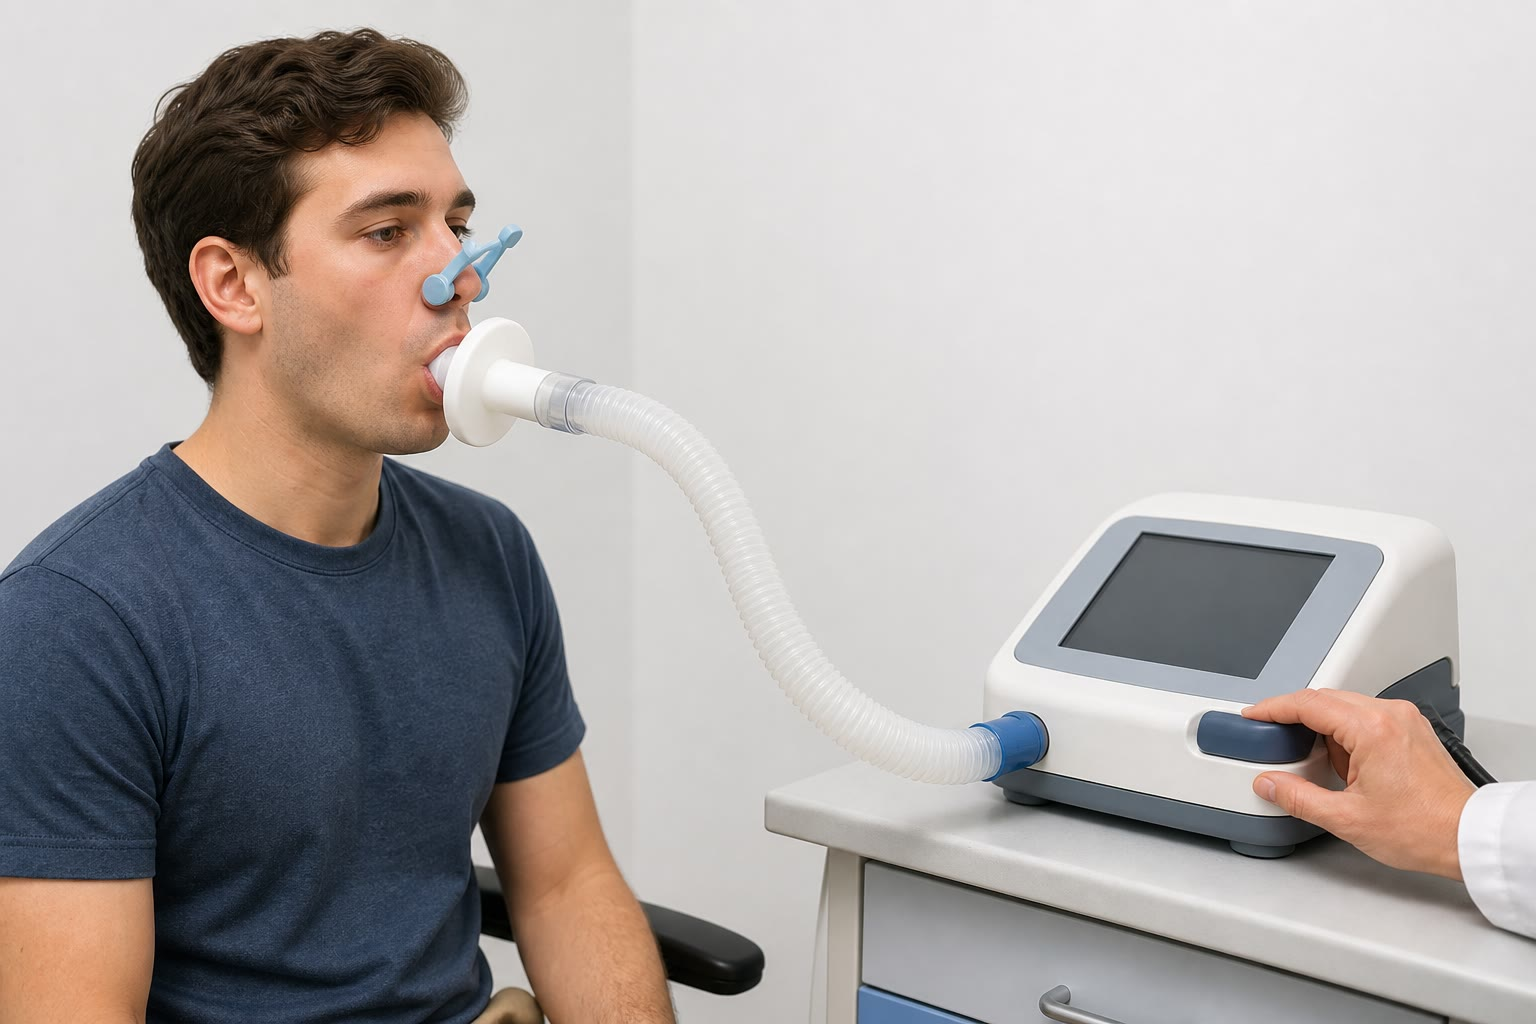
\includegraphics[width=0.58\linewidth]{images/book2/ai/g10-lungs-spirometer.jpg}

{\small 测量肺容积：受试者通过口管在肺量计上呼吸，
鼻孔用夹子夹住，仪器记录
每一次呼吸的体积。}
\end{omfigure}

\section{心脏与体循环、肺循环}

\begin{definition}[心输出量]\label{def:g10:heart-lungs-effort:output}
心脏是由四个腔室构成的双泵。右侧接收
从器官返回的血液，并将其送至肺部
（\emph{肺循环}）；左侧接收从肺部回流的血液，
并将其送至器官（\emph{体循环}）。
腔室之间及出口处的瓣膜使血流只能单向流动。
\emph{心输出量}\index{心输出量} $Q$ 是指
每侧心脏每分钟泵出的血液量，即每次搏动射出的
血量（\emph{每搏输出量} $V_s$）乘以\emph{心率} $f$，
\[
Q = f \times V_s .
\]
静息时，每分钟搏动 $70$ 次，每次泵出 \qty{70}{mL}，约 \qty{5}{L/min}
——相当于全身血量每分钟流过一次。
\end{definition}

\begin{omfigure}
\begin{tikzpicture}[>=Stealth, font=\small,
  ch/.style={draw, thick, rounded corners, minimum width=1.9cm, minimum height=1.0cm, align=center},
  org/.style={draw, thick, rounded corners, minimum width=2.6cm, minimum height=1.0cm, align=center}]
  \node[org, fill=omDef!15] (lungs) at (3.5,3.6) {肺};
  \node[ch, fill=omDef!25] (ra) at (0.7,1.2) {右 \\ 心房};
  \node[ch, fill=omDef!25] (rv) at (0.7,0) {右 \\ 心室};
  \node[ch, fill=omThm!20] (la) at (6.3,1.2) {左 \\ 心房};
  \node[ch, fill=omThm!20] (lv) at (6.3,0) {左 \\ 心室};
  \node[org, fill=omThm!12] (org) at (3.5,-2.8) {肌肉和 \\ 其他器官};
  \draw[->, thick, omDef] (ra) -- (rv);
  \draw[->, thick, omDef, rounded corners=6pt] (rv.west) -- (-1.55,0) -- (-1.55,3.6) -- (lungs.west);
  \node[anchor=east, align=right, omDef] at (-1.7,2.4) {肺 \\ 动脉};
  \draw[->, thick, omThm, rounded corners=6pt] (lungs.east) -- (8.6,3.6) -- (8.6,1.2) -- (la.east);
  \node[anchor=west, align=left, omThm] at (8.75,2.4) {肺 \\ 静脉};
  \draw[->, thick, omThm] (la) -- (lv);
  \draw[->, thick, omThm, rounded corners=6pt] (lv.east) -- (8.6,0) -- (8.6,-2.8) -- (org.east);
  \node[anchor=west, omThm] at (8.75,-1.4) {主动脉};
  \draw[->, thick, omDef, rounded corners=6pt] (org.west) -- (-2.3,-2.8) -- (-2.3,1.2) -- (ra.west);
  \node[anchor=east, omDef] at (-2.45,-1.4) {静脉};
  \node[font=\small, anchor=north, text width=3.2cm, align=center] at (3.5,-3.6) {氧气流出，$\mathrm{CO_2}$ 流入};
  \node[font=\small, anchor=south, text width=3.2cm, align=center] at (3.5,4.2) {氧气流入，$\mathrm{CO_2}$ 流出};
  \draw[thick, dashed, gray] (3.5,2.5) -- (3.5,-1.9);
\end{tikzpicture}

{\small 双循环。蓝色：缺氧血液，由右心泵往
肺部。红色：富氧血液，由左心泵往器官。
左右两侧同步搏动，泵出每分钟相同的
体积。}
\end{omfigure}

\begin{proposition}[运动时的心输出量]\label{prop:g10:heart-lungs-effort:output-exercise}
运动时，心率随输出功率升高，最高可达
约 $220$ 减去年龄（以年计）的数值，每搏输出量也随之增加，
未经训练者约增加一半，经过训练者增幅更大。
青年成人的\omterm{def:g10:heart-lungs-effort:output}{心输出量}从静息时的 \qty{5}{L/min}
升至最大强度时的 \qtyrange{20}{25}{L/min}，
耐力冠军可达 \qty{35}{L/min} 或更高，其每搏输出量
可超过 \qty{180}{mL}。
\end{proposition}
\admitted

\begin{omfigure}
\begin{tikzpicture}
\begin{axis}[
  width=0.86\linewidth, height=5.8cm,
  axis x line=bottom, axis y line=left,
  xmin=0, xmax=320, ymin=0, ymax=210,
  xlabel={机械功率 (W)}, ylabel={心率（次/分）、每搏输出量 (mL)},
  xlabel style={font=\small, at={(axis description cs:0.5,-0.12)}, anchor=north},
  ylabel style={font=\small},
  tick label style={font=\small},
  xtick={0,50,100,150,200,250,300}, ytick={0,50,100,150,200},
  legend style={at={(0.5,-0.3)}, anchor=north, legend columns=3, font=\small, draw=none},
  clip=false,
]
\addplot[thick, omThm, mark=*, mark size=1.5pt] coordinates
  {(0,70) (50,95) (100,120) (150,145) (200,170) (250,190) (300,198)};
\addplot[thick, omDef, mark=square*, mark size=1.5pt] coordinates
  {(0,70) (50,90) (100,105) (150,112) (200,115) (250,115) (300,115)};
\addplot[thick, omMeth, dashed, mark=triangle*, mark size=1.8pt] coordinates
  {(0,4.9) (50,8.6) (100,12.6) (150,16.2) (200,19.6) (250,21.9) (300,22.8)};
\legend{心率, 每搏输出量, 心输出量 (L/min)}
\end{axis}
\end{tikzpicture}

{\small 一名二十岁者在功率递增时的心率、每搏输出量与\omterm{def:g10:heart-lungs-effort:output}{心输出量}。
每搏输出量在中等强度下趋于平稳；超过此强度后，
输出量仅靠心率上升，而心率本身约在
$220 - 20 = 200$ 附近趋于平稳。}
\end{omfigure}

\begin{example}[功率为 \qty{200}{W} 时的输出量]\label{ex:g10:heart-lungs-effort:output200}
由图可知：$f = 170$ 次/分，$V_s = \qty{115}{mL}$，故
$Q = 170 \times 0.115 \approx \qty{19.6}{L/min}$，约为
静息输出量的四倍。心脏每分钟把全身血液总量
泵送四次。
\end{example}

\section{将血液输送到所需之处}

\begin{proposition}[血流的重新分配]\label{prop:g10:heart-lungs-effort:redistribution}
静息时，肌肉约获得\omterm{def:g10:heart-lungs-effort:output}{心输出量}的五分之一；
肠道、肝脏与肾脏约占一半。剧烈运动时，
工作肌肉的小动脉扩张，而肠道与肾脏的小动脉
收缩。肌肉随之获得超过五分之四的输出量，而该输出量本身已增至四倍
——约为 \qty{20}{L/min}，而非
\qty{1}{L/min}，增加了二十倍。大脑所获份额
的绝对量保持不变，皮肤的血流量则上升，以散发热量。
\end{proposition}
\admitted

\begin{omfigure}
\begin{tikzpicture}
\begin{axis}[
  xbar stacked, bar width=15pt,
  width=0.86\linewidth, height=3.8cm,
  axis x line=bottom, axis y line=left,
  xmin=0, xmax=25, xlabel={血流量 (L/min)},
  xlabel style={font=\small, at={(axis description cs:0.5,-0.3)}, anchor=north},
  symbolic y coords={rest, maximal exercise},
  ytick=data, yticklabels={静息, 最大强度运动}, tick label style={font=\small},
  enlarge y limits=0.5,
  legend style={at={(0.5,-0.65)}, anchor=north, legend columns=5, font=\small, draw=none},
]
\addplot[fill=omThm!50, draw=omThm] coordinates {(1.0,rest) (20.5,maximal exercise)};
\addplot[fill=omProp!50, draw=omProp] coordinates {(2.5,rest) (0.9,maximal exercise)};
\addplot[fill=omDef!50, draw=omDef] coordinates {(0.75,rest) (0.75,maximal exercise)};
\addplot[fill=gray!40, draw=gray] coordinates {(0.5,rest) (1.2,maximal exercise)};
\addplot[fill=omMeth!50, draw=omMeth] coordinates {(0.25,rest) (0.65,maximal exercise)};
\legend{肌肉, 肠道与肾脏, 大脑, 皮肤, 其他}
\end{axis}
\end{tikzpicture}

{\small \omterm{def:g10:heart-lungs-effort:output}{心输出量}的去向：静息时（\qty{5}{L/min}）与
最大运动时（\qty{24}{L/min}）的分配。肌肉份额由
五分之一升至五分之四以上；大脑的 \qty{0.75}{L/min} 始终
保持不变。}
\end{omfigure}

\begin{proposition}[氧气的输送与摄取]\label{prop:g10:heart-lungs-effort:extraction}
每升动脉血约携带 \qty{200}{mL} 氧气，
几乎全部与红\omterm{def:g10:cells-common-unit:cell}{细胞}中的血红蛋白结合。静息时
器官每升血液约摄取 \qty{50}{mL}；运动时，
工作肌肉最多可摄取 \qty{150}{mL}，
为静息时的三倍。每分钟的耗氧量等于\omterm{def:g10:heart-lungs-effort:output}{心输出量}
乘以每升的摄取量——因此，输出量的五倍增长与
摄取量的三倍增长共同导致
\cref{ch:g10:exercise-and-energy}中耗氧量的十五倍增长。
\end{proposition}
\admitted

\begin{example}[核对氧气收支]\label{ex:g10:heart-lungs-effort:fick}
静息时：\qty{5}{L/min} $\times$ \qty{50}{mL/L} $= \qty{250}{mL/min}$，即
静息耗氧量。受过训练的学生最大努力时：
\qty{23}{L/min} $\times$ \qty{150}{mL/L} $= \qty{3.45}{L/min}$——即
$\dot V\!\mathrm{O_2}$max 为每千克 \qty{50}{mL/min}，
对应体重 \qty{69}{kg}，恰与上一章的数值相符。
\end{example}

\section{如何控制反应}

\begin{proposition}[神经和激素调节]\label{prop:g10:heart-lungs-effort:control}
心脏和呼吸肌受脑底部的神经中枢驱动。
两组神经连到心脏：一组使心脏减速，静息时起作用；
另一组使心脏加速，并增强每次搏动的力量。运动开始时，
大脑发给肌肉的指令同时传至这些中枢
——心脏在一两次搏动内即加快——，肌肉和关节中的感受器则报告运动。
随后，随着运动持续进行，动脉中的感受器
测量血液中的二氧化碳和酸度，
并调节通气量和心率，使其维持在接近静息时的数值。
肾上腺还分泌一种激素，
\emph{肾上腺素}\index{肾上腺素}，它加强心脏的加速作用，
并使肌肉中的动脉扩张。
\end{proposition}
\begin{proof}[证据]
将动物的减速神经切断，其静息心率由 70 升至约 100；
刺激该神经则使心脏停跳。刺激加速神经
则使心率加倍。告知受试者将要用力时，其心率
在活动前即已上升；让受试者吸入富含二氧化碳的空气，
一分钟内通气量即增加，而
在运动中人为保持其血液二氧化碳不变的人，
在活动开始时通气量仍会增加——预期与校正这两种机制
都是真实存在的。
\end{proof}

\begin{method}[计算氧气的输送]\label{met:g10:heart-lungs-effort:compute}
\begin{enumerate}
  \item 通气量：潮气量 $\times$ 频率。每次呼吸中仅约 70\%
        到达\omterm{def:g10:heart-lungs-effort:ventilation}{肺泡}，其余充满气道。
  \item \omterm{def:g10:heart-lungs-effort:output}{心输出量}：$Q = f \times V_s$，单位为升每分钟，
        若 $V_s$ 以升为单位。
  \item 每分钟耗氧量：$Q \times$（每升血液释放的
        氧气量）。
  \item 流向某器官的血流：其占 $Q$ 的份额。比较绝对血流，
        而非份额——较大输出量中的较小份额，
        可能流经更多的血液。
  \item 检验：耗氧量不能超过 $\dot V\!\mathrm{O_2}$max，
        且 $f$ 不得超过约 $220 - $ 年龄。
\end{enumerate}
\end{method}

\begin{remark}[极限在哪里]\label{rem:g10:heart-lungs-effort:limit}
通气量可超过 \qty{150}{L/min}，离开肺的血液在最大努力时
仍几乎饱和：肺并不是瓶颈。
瓶颈是每搏输出量：它决定每次搏动输送多少血液，
从而输送多少氧气。耐力训练使心脏增大，
每搏输出量随之增加——这正是训练者在同样的 \qty{5}{L/min} 下，
静息心率为 45 而非 70 的原因，
也是 $\dot V\!\mathrm{O_2}$max 随训练升高的原因。
\end{remark}

\section{练习}

\begin{exercise}[$\star$]\label{exo:g10:heart-lungs-effort:1}
计算一人每次呼吸 \qty{0.6}{L}、每分钟十四次时的通气量；
再计算同一人每次呼吸 \qty{2.2}{L}、
每分钟三十五次时的通气量。
\end{exercise}

\begin{exercise}[$\star$]\label{exo:g10:heart-lungs-effort:2}
定义\omterm{def:g10:heart-lungs-effort:output}{心输出量}并给出其公式。求心率为
每分钟 65 次、每搏输出量为 \qty{75}{mL} 时的\omterm{def:g10:heart-lungs-effort:output}{心输出量}。
\end{exercise}

\begin{exercise}[$\star$]\label{exo:g10:heart-lungs-effort:3}
追踪一个红\omterm{def:g10:cells-common-unit:cell}{细胞}从右心房出发、回到右心房的路径，
并写出其经过的心腔与两条循环。
\end{exercise}

\begin{exercise}[$\star$]\label{exo:g10:heart-lungs-effort:4}
根据肺量图，给出潮气量、肺活量
和余气量。
\end{exercise}

\begin{exercise}[$\star$]\label{exo:g10:heart-lungs-effort:5}
一名 16 岁青少年的最大心率是多少？一名 60 岁老人的最大心率是多少？
\end{exercise}

\begin{exercise}[$\star\star$]\label{exo:g10:heart-lungs-effort:6}
根据心率图，求 \qty{100}{W} 与 \qty{300}{W} 时的\omterm{def:g10:heart-lungs-effort:output}{心输出量}，
并求二者之间的倍数关系。
\end{exercise}

\begin{exercise}[$\star\star$]\label{exo:g10:heart-lungs-effort:7}
静息时，肠道和肾脏接受 \qty{5}{L/min} 的 50\%；最大运动时，
则接受 \qty{24}{L/min} 的 4\%。计算两者的血流量。
哪一项变化更大，是份额还是绝对血流量？
\end{exercise}

\begin{exercise}[$\star\star$]\label{exo:g10:heart-lungs-effort:8}
某受试者的\omterm{def:g10:heart-lungs-effort:output}{心输出量}为 \qty{18}{L/min}，其肌肉每升血液
释放 \qty{140}{mL} 的氧气。计算她的耗氧量。
她是否接近受过训练的学生的上限？
\end{exercise}

\begin{exercise}[$\star\star$]\label{exo:g10:heart-lungs-effort:9}
为什么运动时脑部血流量保持在 \qty{0.75}{L/min}，
而肠道血流量在运动中减少了三分之二？请想一想
各器官能够耐受的程度。
\end{exercise}

\begin{exercise}[$\star\star$]\label{exo:g10:heart-lungs-effort:10}
一名训练有素的自行车运动员静息心率为 42，静息输出量为
\qty{5}{L/min}。计算她的每搏输出量，
并与未经训练者的数值比较。
\end{exercise}

\begin{exercise}[$\star\star$]\label{exo:g10:heart-lungs-effort:11}
解释为何心率在赛跑第一步之前就已开始上升，
以及若一名跑者的调节仅靠感知血液中的二氧化碳，
将会发生什么。
\end{exercise}

\begin{exercise}[$\star\star\star$]\label{exo:g10:heart-lungs-effort:12}
两名受试者的最大心率相同，均为 195。其中一人的
最大每搏输出量为 \qty{110}{mL}，另一人为 \qty{160}{mL}。
两人的氧摄取量相同，均为 \qty{150}{mL/L}，计算二者的
\omterm{def:g10:exercise-and-energy:vo2max}{最大摄氧量}，并说明 \cref{rem:g10:heart-lungs-effort:limit} 对
两人训练经历有何预测。
\end{exercise}

\begin{exercise}[$\star\star\star$]\label{exo:g10:heart-lungs-effort:13}
空气中氧气占 21\%。某受试者在最大用力时通气量为 \qty{100}{L/min}，
耗氧量为 \qty{3.5}{L/min}。她实际利用了吸入氧气的多大比例？
其余部分的去向如何？
\end{exercise}

\begin{exercise}[$\star\star\star$]\label{exo:g10:heart-lungs-effort:14}
某药物可阻断加速神经及\omterm{prop:g10:heart-lungs-effort:control}{肾上腺素}对心脏的作用，
将心率限制在 110。预测其对
最大强度下\omterm{def:g10:heart-lungs-effort:output}{心输出量}的影响、对 $\dot V\!\mathrm{O_2}$max 的影响，
以及对患者能完成之活动的影响。
\end{exercise}

\begin{exercise}[$\star\star\star$]\label{exo:g10:heart-lungs-effort:15}
某人身处高海拔地区，其动脉血每升仅携带 \qty{150}{mL} 氧气，
而非 \num{200}。在最大\omterm{def:g10:heart-lungs-effort:output}{心输出量}相同、输送氧气的 75\%
被摄取的条件下，计算 $\dot V\!\mathrm{O_2}$max 的损失百分比。
再提出身体
在随后数周内作出的一种适应。
\end{exercise}

\section{问题：运动负荷试验}

\begin{problem}[{周末问题——心脏病专家的运动试验：
心率、每搏输出量、通气量和氧摄取量随功率升高而测得，
以及它们共同造成的倍增效应}]
\label{pb:g10:heart-lungs-effort:1}
汤姆，17 岁，体重 \qty{68}{kg}，在实验室自行车上蹬踏，
同时记录其心率、通气量和呼出气体。结果如下：

\begin{center}
\begin{tabular}{lccccc}
功率（W） & 0 & 75 & 150 & 225 & 300 \\ \hline
心率（次/分） & 62 & 105 & 140 & 175 & 198 \\
每搏输出量（mL） & 72 & 100 & 116 & 120 & 120 \\
潮气量（L） & 0.5 & 1.2 & 1.8 & 2.3 & 2.6 \\
每分钟呼吸次数 & 13 & 18 & 24 & 32 & 44 \\
每升血液摄取的 $\mathrm{O_2}$（mL） & 52 & 90 & 120 & 145 & 155 \\
\end{tabular}
\end{center}

\medskip
\noindent\textbf{第一部分——心脏。}
\begin{enumerate}
  \item 计算汤姆在各功率下的\omterm{def:g10:heart-lungs-effort:output}{心输出量}。
  \item 在 \qty{300}{W} 时，输出量增至原来的几倍？这一倍数中
        来自心率的部分是多少，来自
        每搏输出量的部分是多少？
  \item 每搏输出量在多大功率以上不再升高？超过该功率后，
        仅靠什么因素使输出量继续增加？
  \item 将汤姆的最大心率与经验法则进行比较。
  \item 他的静息输出量约为 \qty{4.5}{L/min}。若其血容量为 \qty{5}{L}，
        则血液完成一次完整循环在静息时需要多长时间，
        在 \qty{300}{W} 时又需多长时间？
\end{enumerate}

\medskip
\noindent\textbf{第二部分——肺。}
\begin{enumerate}[resume]
  \item 计算各功率下的通气量。
  \item 在 \qty{300}{W} 时，通气量增至原来的几倍？两个因素中，
        潮气量与呼吸频率哪一个贡献更大？
  \item 汤姆的肺活量为 \qty{5.0}{L}。在 \qty{300}{W} 时，每次呼吸
        所用气量占肺活量的比例是多少？
  \item 通气量升高的倍数大于\omterm{def:g10:heart-lungs-effort:output}{心输出量}，这是否说明肺限制了运动表现？
        请结合
        \cref{rem:g10:heart-lungs-effort:limit} 作答。
  \item 每次呼吸中只有 70\% 到达\omterm{def:g10:heart-lungs-effort:ventilation}{肺泡}。计算静息时及
        \qty{300}{W} 时的\omterm{def:g10:heart-lungs-effort:ventilation}{肺泡}通气量。
\end{enumerate}

\medskip
\noindent\textbf{第三部分——氧气。}
\begin{enumerate}[resume]
  \item 根据\omterm{def:g10:heart-lungs-effort:output}{心输出量}与每升血液的氧摄取量，计算汤姆在各功率下的
        耗氧量。
  \item 将 \qty{300}{W} 时的耗氧量以毫升每分钟每千克
        表示。该值是否为 $\dot V\!\mathrm{O_2}$max？若是，
        则受试者属于何种类型？
  \item 耗氧量自静息增至
        \qty{300}{W} 时，增加了多少倍？将其分解为来自心脏的倍数与
        来自氧摄取的倍数。
  \item 取每升氧气的能量为 \qty{20}{kJ}，计算 \qty{300}{W} 时的
        \omterm{def:g10:cell-metabolism:metabolism}{代谢}功率，以及肌肉的效率（机械功率除以高于静息水平的
        \omterm{def:g10:cell-metabolism:metabolism}{代谢}功率）。
  \item 作出耗氧量随机械功率变化的图像，或加以描述。
        该关系是否为线性？耗氧量的上限在哪里？
\end{enumerate}

\medskip
\noindent\textbf{第四部分——调节与结论。}
\begin{enumerate}[resume]
  \item 汤姆坐着等待测试开始时，心率已达到 75。
        请加以解释。
  \item 在 \qty{300}{W} 时，他的动脉血氧饱和度仍为 95\%。这说明
        \omterm{def:g10:heart-lungs-effort:ventilation}{肺泡}的气体交换情况如何，
        以及他的 $\dot V\!\mathrm{O_2}$max 的限制
        位于何处？
  \item 心脏病专家指出，肌肉目前约接受
        \qty{20}{L/min} 的血液。这占\omterm{def:g10:heart-lungs-effort:output}{心输出量}的多大比例，
        静息时其余血流的分配去向如何？
  \item 经过六个月训练，汤姆的最大每搏输出量为
        \qty{140}{mL}，最大心率与摄取率保持不变。计算
        其新的 $\dot V\!\mathrm{O_2}$max。
  \item 陈述结论：汤姆机体放大其静息氧供应所依靠的三个数值
        （心脏、氧摄取、通气），
        以及其中被训练改变的那一个。
\end{enumerate}
\end{problem}
